% =====================================================================
% Template Laporan Tugas — Workshop Deep Learning (Teknik Telekomunikasi ITERA)
% Studi Ablasi RNN, LSTM, GRU vs ANN untuk Prediksi Trafik Seluler
%
% Format IEEE conference dua kolom, MAKSIMAL 6 HALAMAN termasuk referensi.
% Compile: pdflatex main && bibtex main && pdflatex main && pdflatex main
%          (atau: latexmk -pdf main.tex). Bisa juga diunggah ke Overleaf.
%
% Teks bertanda [ ... ] adalah petunjuk: HAPUS dan ganti dengan isi kalian.
% =====================================================================
\documentclass[conference,a4paper]{IEEEtran}
\IEEEoverridecommandlockouts

\usepackage[indonesian]{babel}
\usepackage[utf8]{inputenc}
\usepackage[T1]{fontenc}
\usepackage{cite}
\usepackage{amsmath,amssymb}
\usepackage{graphicx}
\usepackage{booktabs}
\usepackage{siunitx}
\usepackage{xcolor}
\usepackage[hidelinks]{hyperref}
\graphicspath{{gambar/}}

% Penanda petunjuk (hapus pemakaiannya di versi akhir)
\newcommand{\petunjuk}[1]{\textcolor{gray}{[#1]}}

\begin{document}

\title{Studi Ablasi RNN, LSTM, dan GRU dibandingkan ANN untuk Prediksi Trafik Seluler Kota Milan}

% Satu blok per anggota (maks. 3). Hapus blok yang tidak dipakai.
\author{
\IEEEauthorblockN{Muhammad Azriel Patra}
\IEEEauthorblockA{NIM 124400069\\
Teknik Telekomunikasi, ITERA\\
muhammad.124400069@student.itera.ac.id}
}
\maketitle

\begin{abstract}
\petunjuk{150--200 kata. Tuliskan: masalah (prediksi trafik internet per jam), data (Telecom Italia, kotak Duomo dan lokasi kelompok), apa yang diuji (ablasi faktor apa saja, 3 seed), temuan utama dengan angka (misalnya ``GRU terbaik dengan test MAE $x \pm y$, turun $z$\,\% dari acuan''), dan satu kalimat kesimpulan.}
\end{abstract}

\begin{IEEEkeywords}
prediksi trafik seluler, RNN, LSTM, GRU, studi ablasi
\end{IEEEkeywords}

% ---------------------------------------------------------------------
\section{Pendahuluan}
\petunjuk{Mengapa operator perlu meramal trafik per sel? Mengapa model sekuensial (RNN, LSTM \cite{hochreiter1997lstm}, GRU \cite{cho2014gru}) dibandingkan dengan ANN? Apa itu studi ablasi dan mengapa penting? Tutup dengan daftar kontribusi laporan ini (2--3 butir). Maks. 0,5 kolom.}

% ---------------------------------------------------------------------
\section{Data dan Metode}

\subsection{Dataset}
Data yang dipakai berasal dari \textit{Telecom Italia Big Data Challenge}
\cite{barlacchi2015milan} dalam versi agregat per jam dari
\cite{zhang2021fedda}, mencakup trafik seluler kota Milan pada 4 November
sampai 29 Desember 2013. Setiap kotak grid memiliki tiga deret waktu:
aktivitas internet (\textit{net}), panggilan (\textit{call}), dan SMS
(\textit{sms}). Eksperimen utama memakai kotak Duomo (5060), sedangkan uji
generalisasi memakai lokasi kelompok, yaitu [NAMA LOKASI] (kode 9, kotak
[NOMOR KOTAK]). Lokasi tugas ditunjukkan pada Gambar~\ref{fig:peta}.

\begin{figure}[t]
  \centering
  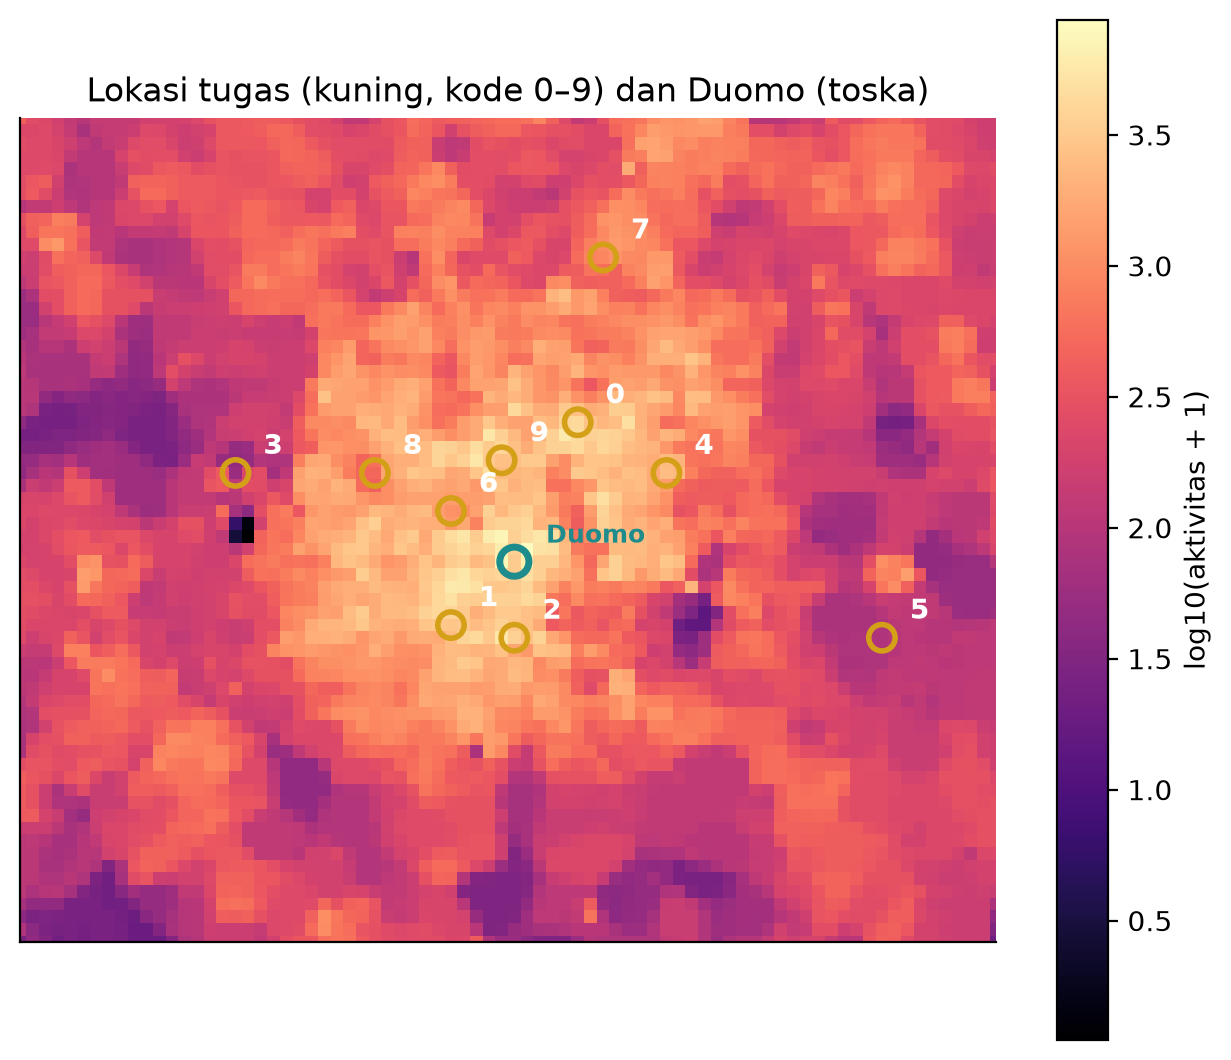
\includegraphics[width=0.85\linewidth]{peta_lokasi_tugas.png}
  \caption{Rata-rata aktivitas internet per kotak di Milan. Lingkaran kuning: lokasi tugas (kode 0--9); lingkaran toska: Duomo.}
  \label{fig:peta}
\end{figure}

\subsection{Pembagian Data dan Praproses}
\petunjuk{Pembagian berdasarkan waktu (train / val / test / Natal), standarisasi dengan statistik sebelum minggu validasi, \textit{windowing}. Jelaskan mengapa data deret waktu tidak boleh diacak.}

\subsection{Model dan Konfigurasi Acuan}
\petunjuk{Uraikan ANN, RNN, LSTM, GRU secara singkat (tanpa menyalin slide). Sajikan konfigurasi acuan dalam Tabel~\ref{tab:acuan}.}

\begin{table}[t]
  \centering
  \caption{Konfigurasi acuan}
  \label{tab:acuan}
  \begin{tabular}{@{}ll@{}}
    \toprule
    Hyperparameter & Nilai acuan \\
    \midrule
    Panjang jendela $W$ & 24 jam \\
    Horizon & 1 jam \\
    Ukuran hidden & ANN 32, RNN 68, LSTM 33, GRU 38 \\
    Jumlah lapisan & ANN 2, rekuren 1 \\
    Fitur & net, call, sms, jam, hari (7) \\
    Optimizer, \textit{learning rate} & Adam, $10^{-3}$ \\
    \textit{Batch size} & 64 \\
    \textit{Early stopping} & \textit{patience} 30, maks.\ 300 epoch \\
    \bottomrule
  \end{tabular}
\end{table}

\subsection{Protokol Ablasi dan Evaluasi}
\petunjuk{Satu faktor diubah setiap kali; daftar faktor dan nilainya (A1--A5 dan dua faktor B pilihan kalian beserta hipotesis awal). Setiap konfigurasi dilatih dengan 3 seed; dilaporkan rata-rata $\pm$ simpangan baku. Metrik: MAE, RMSE, MAPE pada skala asli. Pemilihan konfigurasi terbaik memakai val MAE. Sebutkan perangkat yang dipakai (CPU/GPU) dan total waktu training.}

% ---------------------------------------------------------------------
\section{Hasil}

\subsection{Baseline Naif dan Acuan}
\petunjuk{Tabel baseline naif dan hasil konfigurasi acuan (Bagian 0).}

\subsection{Ablasi Wajib}
\begin{table*}[t]
  \centering
  \caption{Test MAE pada kotak Duomo untuk ablasi A1--A5 (rata-rata $\pm$ simpangan baku, 3 seed). Nilai acuan: $W=24$, \textit{hidden} ANN 32/RNN 68/LSTM 33/GRU 38, 1 lapisan rekuren (ANN 2), $\mathrm{lr}=10^{-3}$, semua fitur.}
  \label{tab:ablasi}
  \footnotesize
  \setlength{\tabcolsep}{4pt}
  \begin{tabular}{@{}llcccc@{}}
    ... (isi tabel dari pesan sebelumnya) ...
  \end{tabular}
\end{table*}
Tabel~\ref{tab:ablasi} merangkum kelima ablasi wajib. Sebagai patokan,
simpangan baku antar seed berkisar $2$--$25$ untuk sebagian besar sel,
sehingga selisih di bawah angka itu tidak dapat dianggap perbedaan nyata.

\textbf{A1 (panjang jendela).} ANN paling sensitif: test MAE turun ke
$271{,}1 \pm 13{,}9$ pada $W=6$ dan memburuk menjadi $402{,}0 \pm 12{,}5$ pada
$W=168$, karena masukan yang makin lebar menambah parameter lapisan pertama
tanpa informasi baru. RNN dan GRU hampir datar terhadap $W$ (RNN $224{,}5$--$233{,}5$;
GRU $237{,}1$--$249{,}8$) dengan selisih di dalam simpangan baku. LSTM terbaik pada
$W=24$ dan memburuk pada jendela lain.

\textbf{A2 (ukuran \textit{hidden}).} Memperbesar \textit{hidden} ke 128
membantu LSTM ($273{,}6 \rightarrow 245{,}6 \pm 6{,}7$) dan GRU
($237{,}2 \rightarrow 220{,}3 \pm 10{,}6$). Pada ANN dan RNN pengaruhnya tidak
konsisten; nilai acuan RNN (68) lebih baik daripada seluruh nilai grid.

\textbf{A3 (jumlah lapisan).} Menambah lapisan tidak membantu. LSTM paling
terpukul: $273{,}6$ (1 lapisan), $308{,}9$ (2), dan $412{,}6 \pm 54{,}2$ (3).
GRU dan RNN memburuk pada 3 lapisan, sedangkan ANN tidak berubah berarti.

\textbf{A4 (\textit{learning rate}).} $10^{-4}$ terlalu kecil untuk semua model
karena \textit{early stopping} berhenti sebelum konvergen (test MAE $287{,}9$--$373{,}5$).
Pada $10^{-2}$, LSTM ($225{,}8 \pm 4{,}2$) dan GRU ($215{,}7 \pm 10{,}9$)
membaik jelas, tetapi ANN menjadi tidak stabil ($309{,}4 \pm 53{,}2$) dan RNN memburuk.

\textbf{A5 (fitur).} Pengaruhnya bergantung model. ANN justru terbaik dengan
fitur \textit{net} saja ($271{,}7 \pm 13{,}9$), sedangkan RNN terbaik dengan
\textit{net+call+sms} ($227{,}6 \pm 2{,}2$) dan GRU dengan semua fitur.
Fitur waktu (jam, hari) tidak memberi keuntungan konsisten.

\subsection{Uji Generalisasi}
\petunjuk{Hasil acuan vs terbaik di lokasi kelompok. Apakah urutan model berubah? Kaitkan dengan pola trafik lokasi tersebut.}

% ---------------------------------------------------------------------
\section{Pembahasan}
\petunjuk{Bagian terpenting. Jangan hanya mengulang angka: jelaskan \emph{mengapa}. Hyperparameter mana yang paling berpengaruh dan mana yang tidak? Apakah perbedaan antar model lebih besar daripada perbedaan antar seed? Apa keterbatasan studi ini (satu kota, 4 minggu train, satu kali pembagian waktu)?}

% ---------------------------------------------------------------------
\section{Kesimpulan}
\petunjuk{3--5 kalimat yang menjawab pertanyaan studi, dengan angka.}

% ---------------------------------------------------------------------
\section*{Kontribusi Anggota}
\begin{tabular}{@{}lp{0.62\linewidth}@{}}
  Nama Anggota 1 & \petunjuk{contoh: Bagian A1--A3, penulisan Hasil} \\
  Nama Anggota 2 & \petunjuk{...} \\
  Nama Anggota 3 & \petunjuk{...} \\
\end{tabular}

\section*{Pernyataan Penggunaan AI}
\petunjuk{Tuliskan alat AI yang dipakai (misalnya ChatGPT, Claude, Copilot) dan untuk apa (memperbaiki kode, merapikan bahasa, dll.). Bila tidak memakai, tulis ``Tidak ada.'' Seluruh angka harus berasal dari run kalian sendiri.}

\section*{Kode dan Data}
Kode, notebook beserta output, dan seluruh hasil run tersedia di \url{https://github.com/muhammad124400069-eng/Muhammad-Azriel-Patra}.

\bibliographystyle{IEEEtran}
\bibliography{references}

\end{document}
